The algorithm proposed by Harms is well designed but is not capable of finding similar user sequences. 
When there is more than one possible interaction to achieve a goal, the method of Harms will create two different sequences for that interaction, 
or worse, will not detect the interaction as a meaningful one at all. For this reason I propose an algorithm that is able to detect similar subsequences.
The basic steps of the algorithm do not differ alot from Harms one. In fact some preprocessing steps and the sequence detection have been altered.
Algorithm \ref{alg:tasktreeoverview} shows the main building blocks and will function as a list and order of contents of this chapter.
\section{Task Tree Generation}

\begin{algorithm}[h]
\floatname{algorithm}{Algorithm}
\begin{algorithmic}
	\Procedure{GenerateTaskTree}{UserSessions}
	\State Harmonize (UserSessions)
	\State Generate Substitution Matrix (UniqueTasks)
	\While{Replaced Tasks} 
	\State Detect Iterations (UserSessions)
	\State Optional: Substitution Matrix Update
	\State Detect Sequences (UserSessions,SubstitutionMatrix)
	\EndWhile
	\EndProcedure
\end{algorithmic}
\caption{Overview over the task tree generation}
\label{alg:tasktreeoverview}
\end{algorithm}

\section{Harmonization}
The user sessions used for task tree generation at the start of this algorithm are available in a non-harmonized form, 
meaning equal task instances may not have the same corresponding task assigned. The harmonization process sets the correct task to those task instances.
Fixing the issue of non-harmonized input data before starting any further steps is crucial since it reduces the number of occuring tasks and makes task instances

comparable by their tasks. Figure \ref{fig:nonharmonized} shows a non-harmonized user session, figure \ref{fig:harmonized} a session where the tasks of equal task instances have been set accordingly.

Another point why this step is important is that it creates a set of unique tasks. This set is needed for the next step of the algorithm, the generation of the substitution matrix.

\begin{figure}[h]
\[
\begin{array}{r|ccccc}
	Task & 1 & 2 & 3 & 4 & 5\\
	\hline
	TaskInstance & A & B & C & A & B\\
\end{array} 
\]
\caption{Non-harmonized user session}
\label{fig:nonharmonized}
\end{figure}

\begin{figure}[h]
\[
\begin{array}{r|ccccc}
	Task & 1 & 2 & 3 & 1 & 2\\
	\hline
	TaskInstance & A & B & C & A & B\\
\end{array} 
\]
\caption{Harmonized user session}
\label{fig:harmonized}
\end{figure}

\section{Task Distance Substitution Matrix}
In section \ref{sec:foundationsubstitutionmatrix} I introduced substitution matrixes in general and what they are good for. 
For this use case I needed to generate one substitution matrix that represents how similar tasks are. 
The score of two tasks in the \textit{task distance substitution matrix} is defined as follows:
\begin{definition}
	\item Let a and b be two tasks
	\item Let S(a,b) be the score for substituting task a with task b. The higher the value of S is, the more similar are the tasks a and b and vice versa.
\end{definition}

To calculate the score, three cases have to be considered:
\begin{itemize}
	\item Similarity of two event-tasks
	\item Similarity of an event-task and a non-event-task
	\item Similarity of two non-event-tasks
\end{itemize}

\subsection{Event-Task Event-Task Similarity}
The first idea was to calculate the score of the matrix based on the distance between the absolute coordinates of the events-tasks. 
There are a few problems with this approach: First, not all event-tasks may have absolute coordinates. 
The second problem with this method is that in graphical user interfaces events may still be very similar, even if they have a large absolute distance.
An example for such a case would be a web formular with many fields to fill out. 
TODO: Maybe Screenshot here?
Those fields take space which would result in large distances between them although the event-tasks all belong to a single formular.
The solution to this problems is to make use of a grouping of elements the designer of the GUI already did: The GUI-Model (see section \ref{sec:foundationguiandguimodel}).
Elements of a GUI that belong to one semantic task can usually be found in some kind of container that groups those elements together. Therefore the basis for my 
distance calculation is the distance in the GUI-Model, as defined in \ref{def:guimodeldistanceee}. 

\begin{definition}
	\item Let a and b be events-tasks
\begin{equation*}d(a,b) = d(b,a) = \text{the distance in the GUI model of the targets of event-tasks a and b.}
\end{equation*}
\label{def:guimodeldistanceee}
\end{definition}

Since the GUI model is a tree, the distance of two targets in a GUI can easily be calculated by finding the common ancestor of the targets and summing up the number of nodes from both the events to this ancestor, including the ancestor.
\begin{figure}
\begin{center}
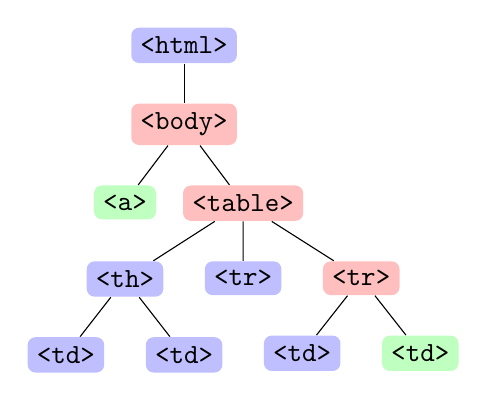
\begin{tikzpicture}[
    fact/.style={rectangle, draw=none, rounded corners=1mm,
        text centered, anchor=north, text=black, fill=blue!25},
    redcolor/.style={rectangle, draw=none, rounded corners=1mm,
        text centered, anchor=north, text=black, fill=red!25},
    greencolor/.style={rectangle, draw=none, rounded corners=1mm,
        text centered, anchor=north, text=black, fill=green!25},
    level distance=0.5cm, growth parent anchor=south]

\node (Fact01) [fact] {\texttt{<html>}} [-]
    child{
        node (kolor4) [redcolor] {\texttt{<body>}}
        child{
            node (color1) [greencolor] {\texttt{<a>}}
        }
        child{
            node (Fact04) [redcolor] {\texttt{<table>}}
            child{
                node (Fact05) [fact] {\texttt{<th>}}
                child{
                    node (fact5) [fact] {\texttt{<td>}}
                }
                child{
                    node (Fact07) [fact] {\texttt{<td>}}
                }
            }
	    child{
                node (Fact05) [fact] {\texttt{<tr>}}
	    }	
            child{
                node (color3) [redcolor] {\texttt{<tr>}}
                child{
                    node (Fact10) [fact] {\texttt{<td>}}
                }
                child{
                    node (color2) [greencolor] {\texttt{<td>}}
                }
            }
        }
    }   
;
 
\end{tikzpicture}
\end{center}	
\label{fig:guimodeldistance}
\caption{A HTML GUI model with two nodes (green) the distance will be calculated for.  The number of red nodes is the distance between the green nodes. The common anchestor is the \texttt{<body>} element.}

\end{figure}
Figure \ref{fig:guimodeldistance} shows a GUI model with two elements and their common ancestor. 


\subsection{Event-Task Non-Event-Task Similarity}
It takes a bit more effort to calculate the substitution score if one task is a non-event-task. 
The reason is that the non-event tasks do not represent a simple event anymore. Therefore they do not possess a target in the GUI.
A possible solution is to recursively visit every child of the non-event-task, gather all event tasks and then calculate the mean distance from each of those tasks to the event-task the distance shall be calculated to.
Formally, definition \ref{def:guimodeldistanceee} has to be modified so that it covers non-events as well:

\begin{definition}
%	\item Let a and b be events-tasks, then:
%\begin{equation*}d(a,b) = d(b,a) = \text{be the distance in the GUI model of the targets of event-tasks a and b.}
%\end{equation*}
	\item Let c be a non-event-task
	\item Let E be the set containing all event-tasks that can be recursively found in c.
	\item with definition \ref{def:guimodeldistanceee} it is possible to define d as
\begin{equation*}
	d(a,c) = d(c,a) = \frac{\sum_{\forall x \in E} d(a,x)}{|E|}
\end{equation*}
\label{def:guimodeldistanceene}
\end{definition}

\subsection{Non-Event Non-Event Similarity}
With Definition \ref{def:guimodeldistanceene} it is simple to compute the distance for two tasks since all that is to do now is to repeat the procedure of finding all event-task children of one task, calculate the distances to the other task and use the mean distances as the total distance.
The definition of d can be extended so it accepts two non-event-tasks:

\begin{definition}
	\item Let c and d be non-event-tasks 
	\item Let E be the set containing all event-tasks that can be recursively found in c.
	%\item Let F be the set containing all event-tasks that can be recursively found in d.
	\item with definition \ref{def:guimodeldistanceene} it is possible to define d as
	\begin{equation*}
		d(c,d) = d(d,c) = \frac{\sum_{\forall x \in E} d(x,d)}{|E|}
	\end{equation*}
\label{def:guimodeldistancenene}
\end{definition}
\subsection{Score}
Now that I defined the distance for three cases it is possible to compute the score $S$ of two tasks.
\begin{definition}
	\item Let U be the set of unique tasks occurring in the user sessions
	\item Let k be a constant that defines the maximal score 
	\item For each tupel $i,j \in U$ 
\begin{equation*}
		 S(i,j) = -1*d(i,j)+k
	\label{eq:subscore}
\end{equation*}
\end{definition}

The k constant should be chosen dependent on the underlying GUI model. A large k should be chosen for very deeply, nested GUI models, whereas for flat GUI models a smaller k seems better. 

\section{Iteration Detection and Substitution Matrix Update}
The iteration detection from Harms is also suitable for my algorithm was not altered in any way. It reliably detects iterations and replaces them in the user sessions.
Before the sequence detection can come to play the substitution matrix should be updated since there were new iteration tasks created during iteration detection. Those new tasks are stored in a set that contains all newly created tasks.
The update process differs just a little from the generation process with the only difference beeing that just the distances between the newly created tasks to the current set of unique tasks is as well as the distances between the newly created tasks are computed.
After the matrix has been updated, the newcly created tasks are merged with the set of unique tasks and then emptied.
The whole step of updating the matrix is currently implemented but not used. Instead, each score between an event-task to a non-event-task and therefore all scores between non-event-tasks are defined as zero due to perfomance issues.
More details on this issue can be found in section TODO: REF HERE.

\section{Sequence Detection}
As i figured out at the beginning of this chapter, the sequence detection is the part of the algorithm that varies the most from Harms approach.
It is itself separated in three in steps:
\begin{itemize}
	\item The search for significant regions
	\item The model generation
	\item The sequence replacement
\end{itemize}

\subsection{Search for significant regions}		
\begin{itemize}
	\item For sequence detection a method called alignments is used
	\item It can be used for approximate string matching. 
	\item This is useful for this problem, because we also want to detect similar interactions of different users, not just equal interactions
	\item align each user session with any other user session (section alighments)  (if not mentioned, mention complexity of $O(n^2)$
\end{itemize}

\paragraph{Smith Waterman Algorithm For Repeated Matches}
\begin{itemize}
	\item Modified Version of the smith waterman algorithm
	\item Finds all local alignments of two sequences that reach a threshold score, not just the best
	\item Uses dynamic programming
	\item Exact method, not heuristic
	\item Two sequences: 
	\item y: pattern
	\item x: sequence in which we search all subsequences of y repeatedly
	\item Final aligment: x has matched and unmatched regions
	\item Uses matrix (dynamica programming matrix) where each cell stores the best score for aligning the elements at the position the cell represents
	\item Advantage: Possible alignments with less score do not need to be calculated recursively
	\item Score of a matched region: sum of all scores for each position minus the score threshold 
	\item first row has a different meaning than in basic Smith waterman (score of the last matched subsequence)
	\item Definitions:
	\item F is the dynamic programming matrix
	\item S is the score of the substitution matrix
	\item g is the gap penalty
\end{itemize}

\subparagraph{Intialization}:
	\begin{itemize}
		\item \[F(0,0) = 0\]
%		\item Fill first col with 0, 
	\end{itemize}

\subparagraph{Recursion}
	\begin{itemize}
		\item Build dynamic programmic matrix
		\item  \[F(i,0) = max \left\{ \begin{array}{lr}F(i-1,0)&\\F(i-1,j)-T& j=1,\dots,m\end{array}\right. \]
		\item  \[F(i,j) = max \left\{ \begin{array}{lr}F(i,0),\\F(i-1,j-1)+S(x_i,y_i),\\F(i-1,j)-g,\\F(i,j-1)-g\end{array}\right.\]
		\item Explain each choice we can take here
		\item Store every choice we took
	\end{itemize}

\subparagraph{Traceback}
Go back from the addition cell in the first row to first cell to get alignment
\includegraphics[width=\textwidth]{chapters/approach/smithwatermanrepeated.png}
%	\[
%	\begin{pmatrix}
%                   & - &   & A &   & C &   & A &   &  C & A & C & T & A \\
%	         - & \color{blue}0 & 0 & 0 & 0 & 0 & 0 & 0 & 0 & 0 \\
%	         A & 0 & \color{blue}2 & 1 & 2 & 1 & 2 & 1 & 0 & 2 \\
%	         G & 0 & \color{blue}1 & 1 & 1 & 1 & 1 & 1 & 0 & 1 \\
%	         C & 0 & 0 & \color{blue}3 & 2 & 3 & 2 & 3 & 2 & 1 \\
%	         A & 0 & 2 & 2 & \color{blue}5 & 4 & 5 & 4 & 3 & 4 \\
%	         C & 0 & 1 & 4 & 4 & \color{blue}7 & 6 & 7 & 6 & 5 \\
%	         A & 0 & 2 & 3 & 6 & 6 & \color{blue}9 & 8 & 7 & 8 \\
%	         C & 0 & 1 & 4 & 5 & 8 & 8 & \color{blue}11 & \color{blue}10 & 9 \\
%	         A & 0 & 2 & 3 & 6 & 7 & 10 & 10 & 10& \color{blue}12
%	\end{pmatrix}
%	\]

\subparagraph{Scoring}
Describe how each match is scored

\subparagraph{Match retrival}
	\begin{itemize}
		\item retrieve matches that reach a defined threshold from each alignment pair
		\item Due the nature of this algoritm, all matches that can be found have this minimal score
		\item A match consists of 2 sequences of numbers. 
		\item for each found match:
		\item Search match in all user sessions
		\item From the most to the least found match:
	\end{itemize}
\subsubsection{Model generation}
	\begin{itemize}
		\item Generate Model From Match is done the following way:
		\item For each position of the Match: 
		\item (remind, that each match has 2 Sequences of aligned numbers)
		\begin{itemize}
			\item If Both numbers are equal: The model at this position is the Task refered by this number
			\item If one sequence has a gap at this position: The other EventTask is inserted as an optional
			\item If both numbers differ a selection is inserted. Which kind of selection depends on what the following task is. We don't want to have 2 selections next to each other, instead, create one selection and add each sequence as a sequence
			\begin{itemize}
				\item If the next position also would be a selection, the selection has 2 sequences as a child. those sequences consists of the tasks of each sequence of the match until there is no more selection found 
				\item If the next position is something else we just have a single selection, just add the tasks of the match at this position as childs to the selection
				\item (This description here is really bad, will need some examples)
			\end{itemize}
		\end{itemize}
	\end{itemize}

\subsubsection{Replacement}
	\begin{itemize}
		\item Replace each model in the user sessions
	\end{itemize}

\subsection{Repetition}



